%! TEX program=pdflatex
%! BIB program=bibtex
\documentclass[a4paper,twocolumn]{article} % Document type
\usepackage{times} % Use  Font Times New Roman
\ifx\pdfoutput\undefined
    % Use old Latex if PDFLatex does not work
   \usepackage[dvips]{graphicx} % To get graphics working
   \DeclareGraphicsExtensions{.eps} % Encapsulated PostScript
 \else
    %Use PDFLatex
   \usepackage[pdftex]{graphicx}% To get graphics working
   \DeclareGraphicsExtensions{.pdf,.jpg,.png,.mps} % Portable Document Format, Joint Photographic Experts Group, Portable Network Graphics, MetaPost
   \pdfcompresslevel=9
\fi

\usepackage{amsmath,amssymb}   % Contains mathematical symbols
\usepackage[ansinew]{inputenc} % Input encoding, identical to Windows 1252
\usepackage[english]{babel}    % Language
%\usepackage[round,authoryear]{natbib}  %Nice author (year) citations
\usepackage[square,numbers]{natbib}     %Nice numbered citations
%\bibliographystyle{unsrtnat}           %Unsorted bibliography
\bibliographystyle{plainnat}            %Sorted bibliography
\usepackage{caption}
\addtolength{\topmargin}{-30mm}% Removes 30mm from the top margin
\addtolength{\textheight}{30mm}% Adds it to the text height
\usepackage{multirow} % Create table with multirow
\usepackage{hyperref} % Generate internal hyperlinks for figure, table, reference
\hypersetup{
		colorlinks=true,
		linkcolor=blue,}
\usepackage{indentfirst} %首段縮排
 \usepackage{lscape}
 \usepackage{comment}
  \usepackage[left=2.0cm, right=2.0cm, top=2.0cm, bottom=2.0cm]{geometry}

\begin{document}               % Begins the document
	\title{The Experiment of Leukemia Classification using SVMs with Feature Selection Methods}
	%\title{Evaluating SVM Algorithms for Bioinformatics Gene Expression Analysis}
	\author{}
	\date{2019-01-09} % Follow the ISO8601 standard
	
	\maketitle                     % Generates the title
	\section*{Abstract}
	\label{sec:abs}
	\noindent {\bf Motivation}: Feature selection methods are used to optimized SVM method for better classifying the unknown tissue sample which are applied on leukemia cancer datasets.\\
	{\bf Problem}: The MSFS method claims to have better accuracy than the others feature selection. Since, the paper give only brief explanation about the details, the method could not be confirmed. And also, the lymphoma datasets do not have concrete clarity of the data as diverse as investigation that has been conducted. Thus, we only focused on leukemia datasets.\\
	{\bf Approach}: We performed the SVM by evaluating several feature-selection with different kernel method, and evaluated the weighted average to compared it with the claimed accuracy.\\
	{\bf Results}: Got similar accuracy as the original paper, but with significantly less feature number. RFE models predict better than SFS, and far more effective.\\
	{\bf Conclusion}: RFE with linear classification kernel is the best model for Leukenia dataset.
	
	\section*{Introduction}
	\label{sec:intro}
	Support vector machines (SVMs) are supervised learning method which broadly used in many domains which has been successfully applied and developed in bioinformatics fields. It is one of the state-of-the-art kernel-based machine learning techniques which is suitable for tissue classification and prediction. For instance, the classification of microarray gene expression data. 
	Microarray technologies are utilized to estimate the survival time and risk of cancer metastasis or recurrence based on the patient's genotypic microarray data. Microarray data typically high dimensionality and relatively few examples characterized in gene expression data, which make it impossible to do it manually. Thus, SVMs are utilized to obtain classification models with such high dimensional data. The main focus is the feature selection in order to reduce the dimensionality of dataset. Such that, the better accuracy results can be obtained.
	
	\begin{comment} %SVMs in Bioinformatics 不顯示
    	\subsection*{SVMs in Bioinformatics}
   % 	Figure \ref{fig:Fig1} shows an illustration about how SVMs classify of microarray gene %expression data.
    	The nodes (the vectors) that define the hyperplane, can be regarded as the support vectors, while the hyperplane represents as a plane that maximize the margin between the two classes. When the hyperplane completely separates the vectors (cases) into non-overlapping classes, it can be considered as an ideal SVMs. In the experiment, genes represented by nodes which has high dimension. While feature selection eliminated the redundant noise of the genes to obtain the better accuracy results. The goal of this method is to better classifying the ALL (acute lymphocytic leukemia) and AML (acute myelocytic leukemia) based-on leukemia cancer data sets which are all acute leukemia patients contain 72 samples with 7128 genes each of sample.
	\end{comment}
	
	\section*{Problem description}
	\label{sec:prob}
	The gene expression analysis for classifying and predicting cancer in tissue samples is an important topic on bioinformatics. This paper \cite{Bhat2017EvaluatingSA} claims that SVM-MSFS (modified successive feature selection) is better than the other feature selection methods mentioned in the article on classification accuracy (up to 95 \%), but there were no detailed description provided in the article.
	
	\section*{Data description}
	\label{sec:data}
	
	We focused on the Leukemia dataset, which contains 7128 genes taken from 72 samples. Two variants of leukemia, ALL (acute lymphocytic leukemia) and AML (acute myelocytic leukemia), were labeled before training (Table \ref{tab:tvar}). The original data were transposed for easier processing with Python. During training process, the order of data within the dataset was randomized before every iteration to avoid bias.
	
		\begin{table}[h]
		\caption{Sample numbers for 2 different variants of leukemia, ALL and AML.}\label{tab:tvar}
		\begin{tabular}{ ccc } % This create table with all grid lines and put text by center
			\hline
			Variant name &  Numbers\\
			\hline
			Acute Lymphoblastic Leukemia (ALL) & 47\\
			Acute Myeloid Leukemia (AML) & 25\\
			\hline
		\end{tabular}
	\end{table}
	
	\section*{Methods}
	\label{sec:meth}
	\begin{itemize}
		\item SVM-Recursive Feature Elimination (RFE)\\
		SVM-RFE removes redundant genes based on weight-based saliency analysis. Genes connected to important features receive large absolute values of weight, which will later being conserved, and those genes that receive small absolute values of weight will be removed, and the new gene subset is formed for further analysis.
		
		\item SVM-Successive Feature Selection (SFS)\\
		SVM-SFS processes the features in a set one at a time, and found that the suitable values of x taken due to the memory constraints is equal or less than 10, and the rank of features will be the output of the algorithm. In the successive level, the feature is dropped once at a time, a subset of feature is obtained, and the best subset of the feature is processed to the next level after evaluation.
		
	\end{itemize}
	
    We applied RFE with linear regression kernel and tried linear, RBF (radial basis function) and polynomial classification kernel. As for SFF we tested knn (k-nearset neighbor) and logistic regression kernel with linear classification kernel (Table \ref{tab:meth}). The flowchart of how the SVM feature selection algorithms work is shown in Figure \ref{fig:Flow}.\newline
    
    The suggested feature number for the model to select by \cite{Bhat2017EvaluatingSA} is 140, and number of training data and testing data are 38 and 34, suggested by \cite{Golub531}.But the feature number should not excess sample number significantly like this setting, so we decrease the selected feature number from 10 feature to 70 features, and compare the performance of the model. Since the total number of the samples are quite small, the combination of the training data acts as major factor to the accuracy of the prediction. In order to eliminate the influence of the training data configuration, we randomized the order all the 72 samples in every iteration, but the number of training data and testing data remain the same, 38 and 34. In each iteration, we calculate the Matthews correlation coefficient (MCC), on both training data and testing data.
    
    \begin{figure}[h]
		\begin{center}
			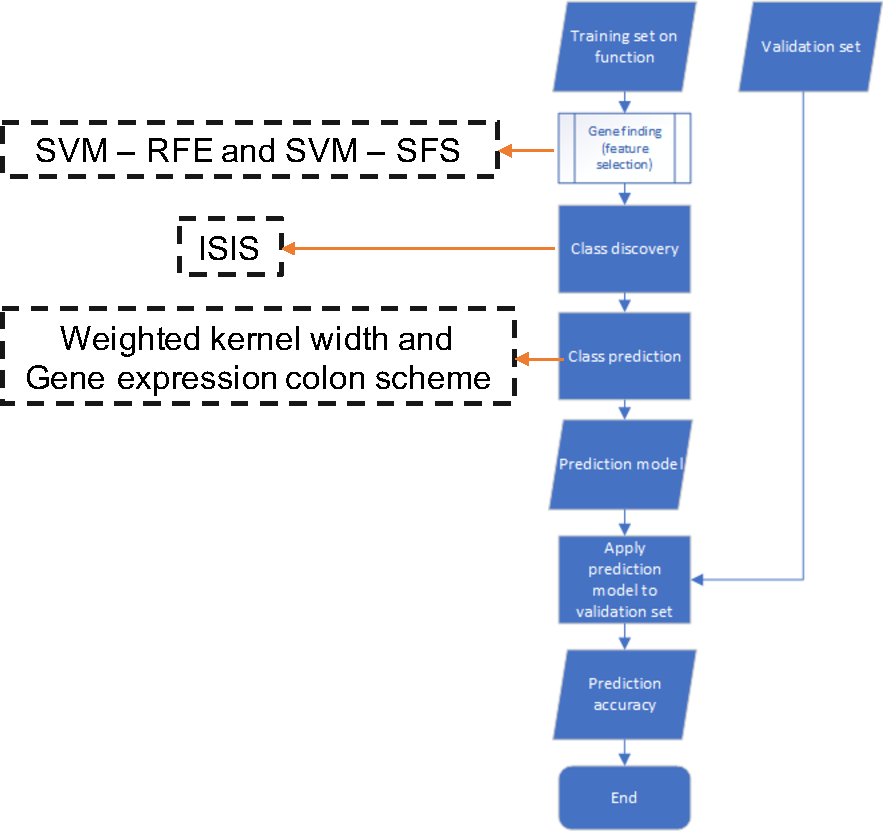
\includegraphics[width=200pt]{FSA_flowchart.pdf}
			\caption{Flowchart of the SVM feature selection algorithm.}
			\label{fig:Flow}
		\end{center}
	\end{figure}

	\section*{Results and Discussions}
	\label{sec:res}  
	
	For RFE method, the performance of polynomial classification kernel is the worst among all classification kernels. No matter how many features and how many iterations, the model can only recognize one class. In this case, the model can not make any prediction at all, so we omit polynomial classification kernel in further comparison. As for linear kernel, the MCC of training data are 1.0 (Figure \ref{fig:Train_RFE_Linear}), and MCC of testing data rise with respect to feature number (Figure \ref{fig:Test_RFE_Linear}). With RBF kernel, both the MCC of training data (Figure \ref{fig:Train_RFE_RBF}) and testing data (Figure \ref{fig:Test_RFE_RBF}) vary, but with all of them approach to 1 with increasing feature number.\newline
	
	For SFS method, the time required for computation is far more than RFE, and the MCC of trainind data are all very close to 1.0 (Figure \ref{fig:Train_SFS_Logistic}, Figure \ref{fig:Train_SFS_KNN}). Though KNN regression method takes even more time than logistic regression method, the MCC of KNN on testing data (Figure \ref{fig:Test_SFS_KNN}) are a bit less than logistic one (Figure \ref{fig:Test_SFS_Logistic}).

	\section*{Conclusion}
	\label{sec:conc}
	
	In Figure \ref{fig:Comparison}, we compare the weighted accuracy of our four method with the author's result. The selected feature number are 140 in every method, and the accuracy is the average of the 50 iteration of each method. The accuracy of RFE in our results are a little bit better than the author's. But the accuracy of SFS, which the author claimed is higher than RFE, turned out to be worse than RFE in our result. Especially for SFS with KNN regression kernel, the accuracy is 10\% less than the paper's.\newline
	
	
	The feature number effects accuracy of RFE with RBF kernel considerably. In Figure \ref{fig:RFE_accuracy}, only when feature number exceeded 40 can the average accuracy got better than 90\%. But the RFE accuracy with linear kernel seems similar in every feature number. Also in Figure \ref{fig:SFS_accuracy}, both Knn and logistic regression kernel show no relationship between accuracy and feature number.
	
	
	
	\begin{figure}[htp]
		\begin{center}
			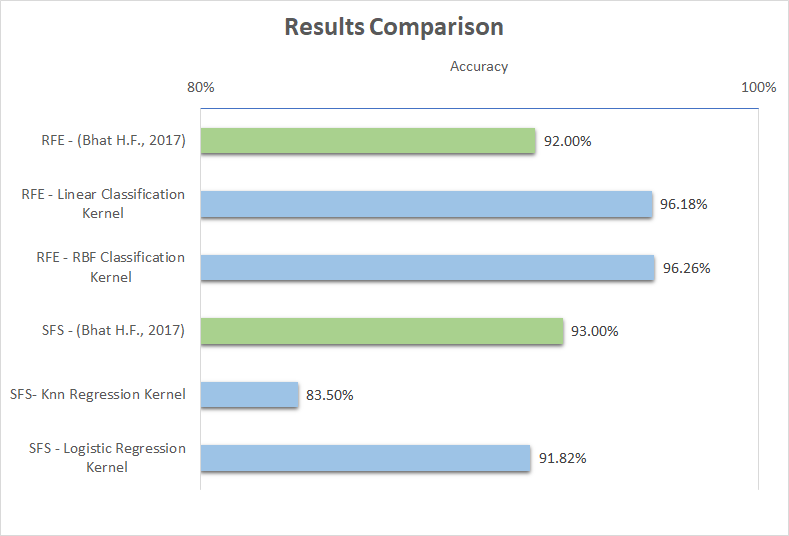
\includegraphics[width=230pt]{comparison.png}
			\caption{Accuracy comparison between our result and the author's result}
			\label{fig:Comparison}
		\end{center}
	\end{figure}
	
	
 \bibliography{reference} \label{sec:ref}

	\newpage
\onecolumn
\section*{Appendix}
	%	\begin{figure}[htp]
	%	\begin{center}
	%		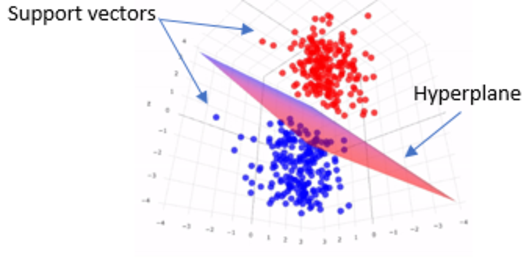
\includegraphics[width=200pt]{Fig1.pdf}
	%		\caption{Illustration of how SVMs classify the microarray gene expression data.}
	%		\label{fig:Fig1}
	%	\end{center}
	%  \end{figure}
	
\begin{table*}[h]
	\caption{The methods we apply to conduct feature selection and class prediction.}\label{tab:meth}
	\begin{tabular}{lll} %This create table with only the grid lines at where you use \hline and put text by left
		\hline
		& Regression kernel & Classification kernel\\
		\hline
		\multirow{3}{*}{RFE} & Linear & Linear\\
		& Linear            & RBF\\
		& Linear  & Polynomial   \\
		\hline
		\multirow{2}{*}{SFS} &KNN & Linear\\
		& Logistic                 & Linear\\
		\hline
	\end{tabular}
\end{table*}

		\begin{figure*}[h]
		\begin{center}
			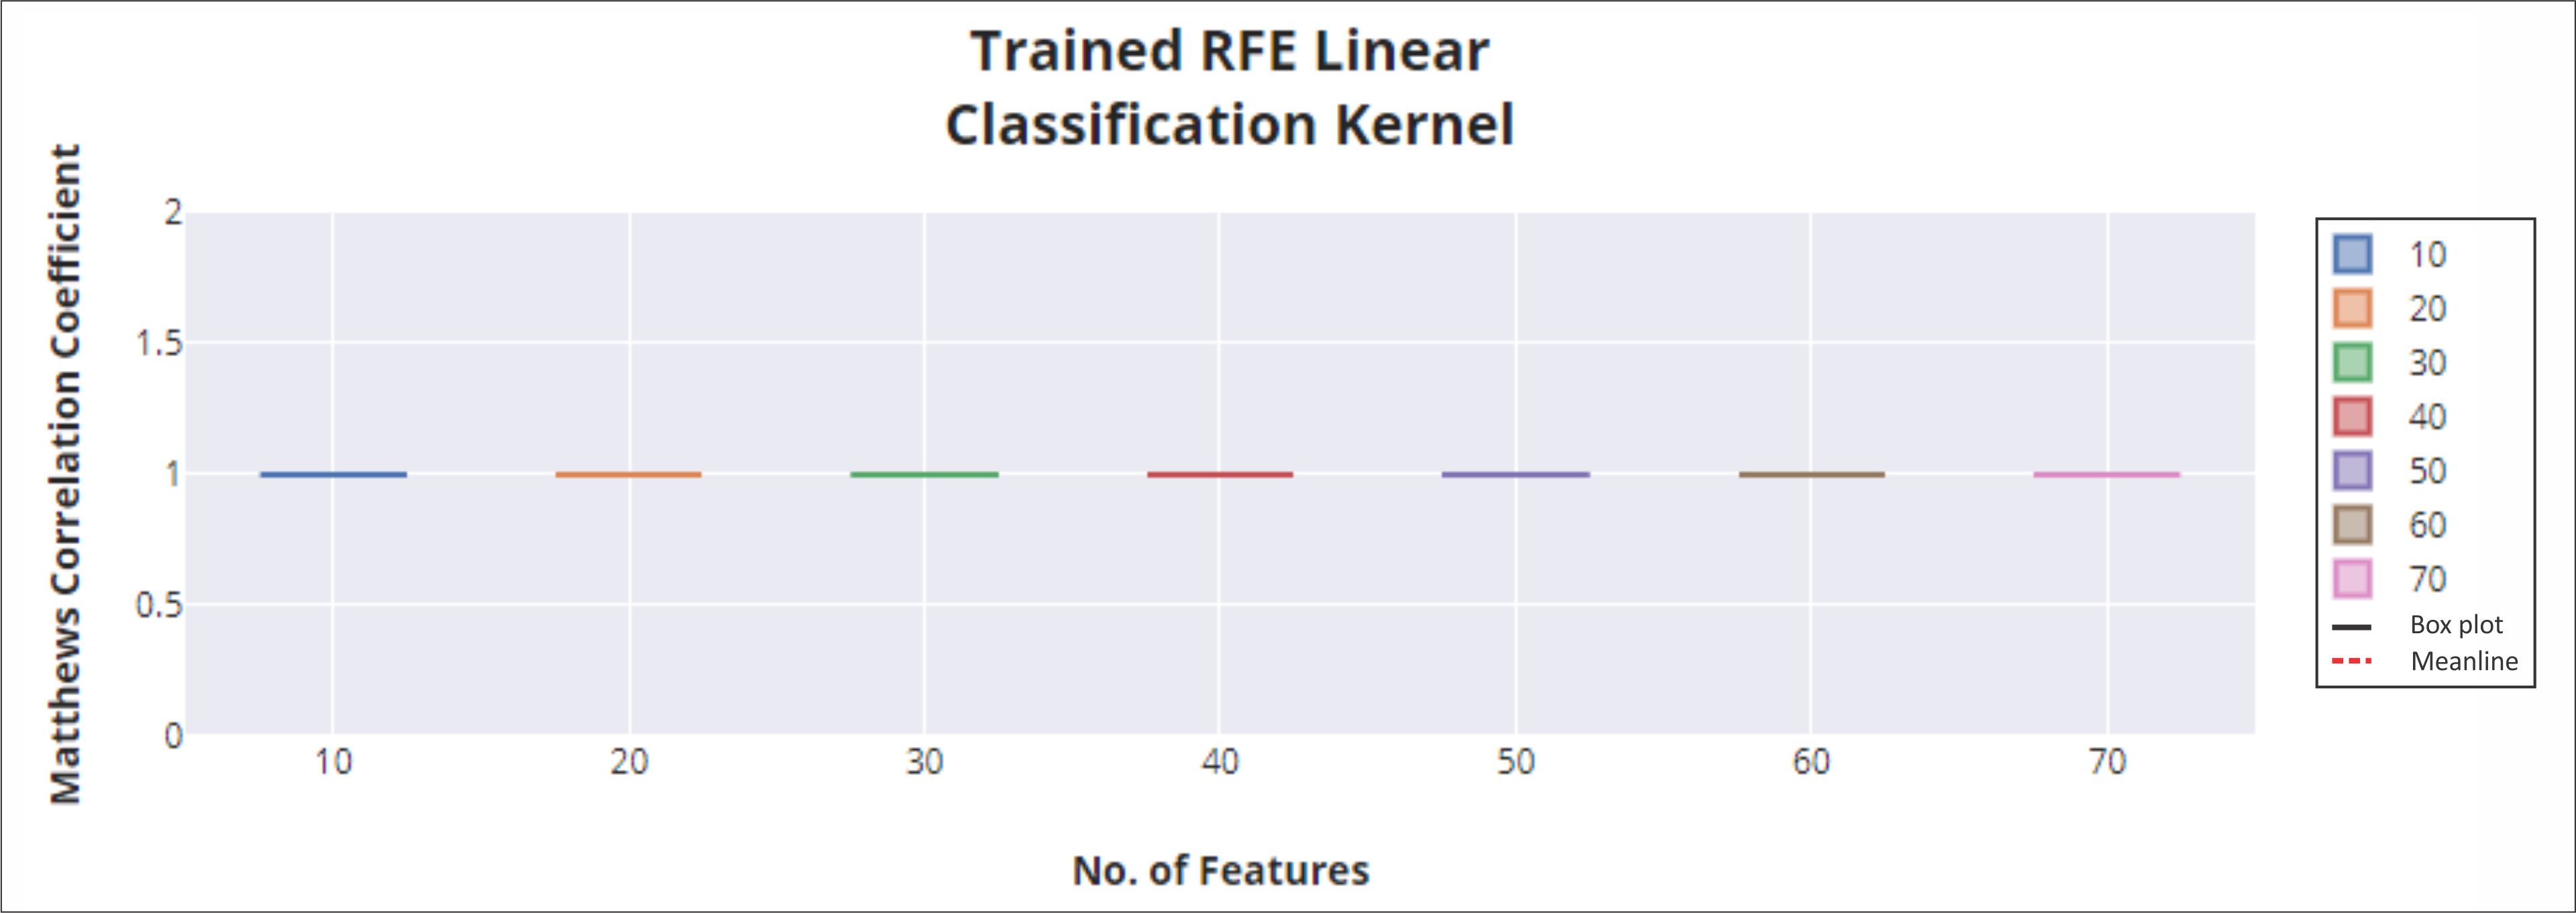
\includegraphics[width=500pt]{Trained_RFE_Linear_Classification_Kernel.PNG}
			\caption{Training data: RFE linear classification kernel}
			\label{fig:Train_RFE_Linear}
		\end{center}
	\end{figure*}

		\begin{figure*}[h]
		\begin{center}
			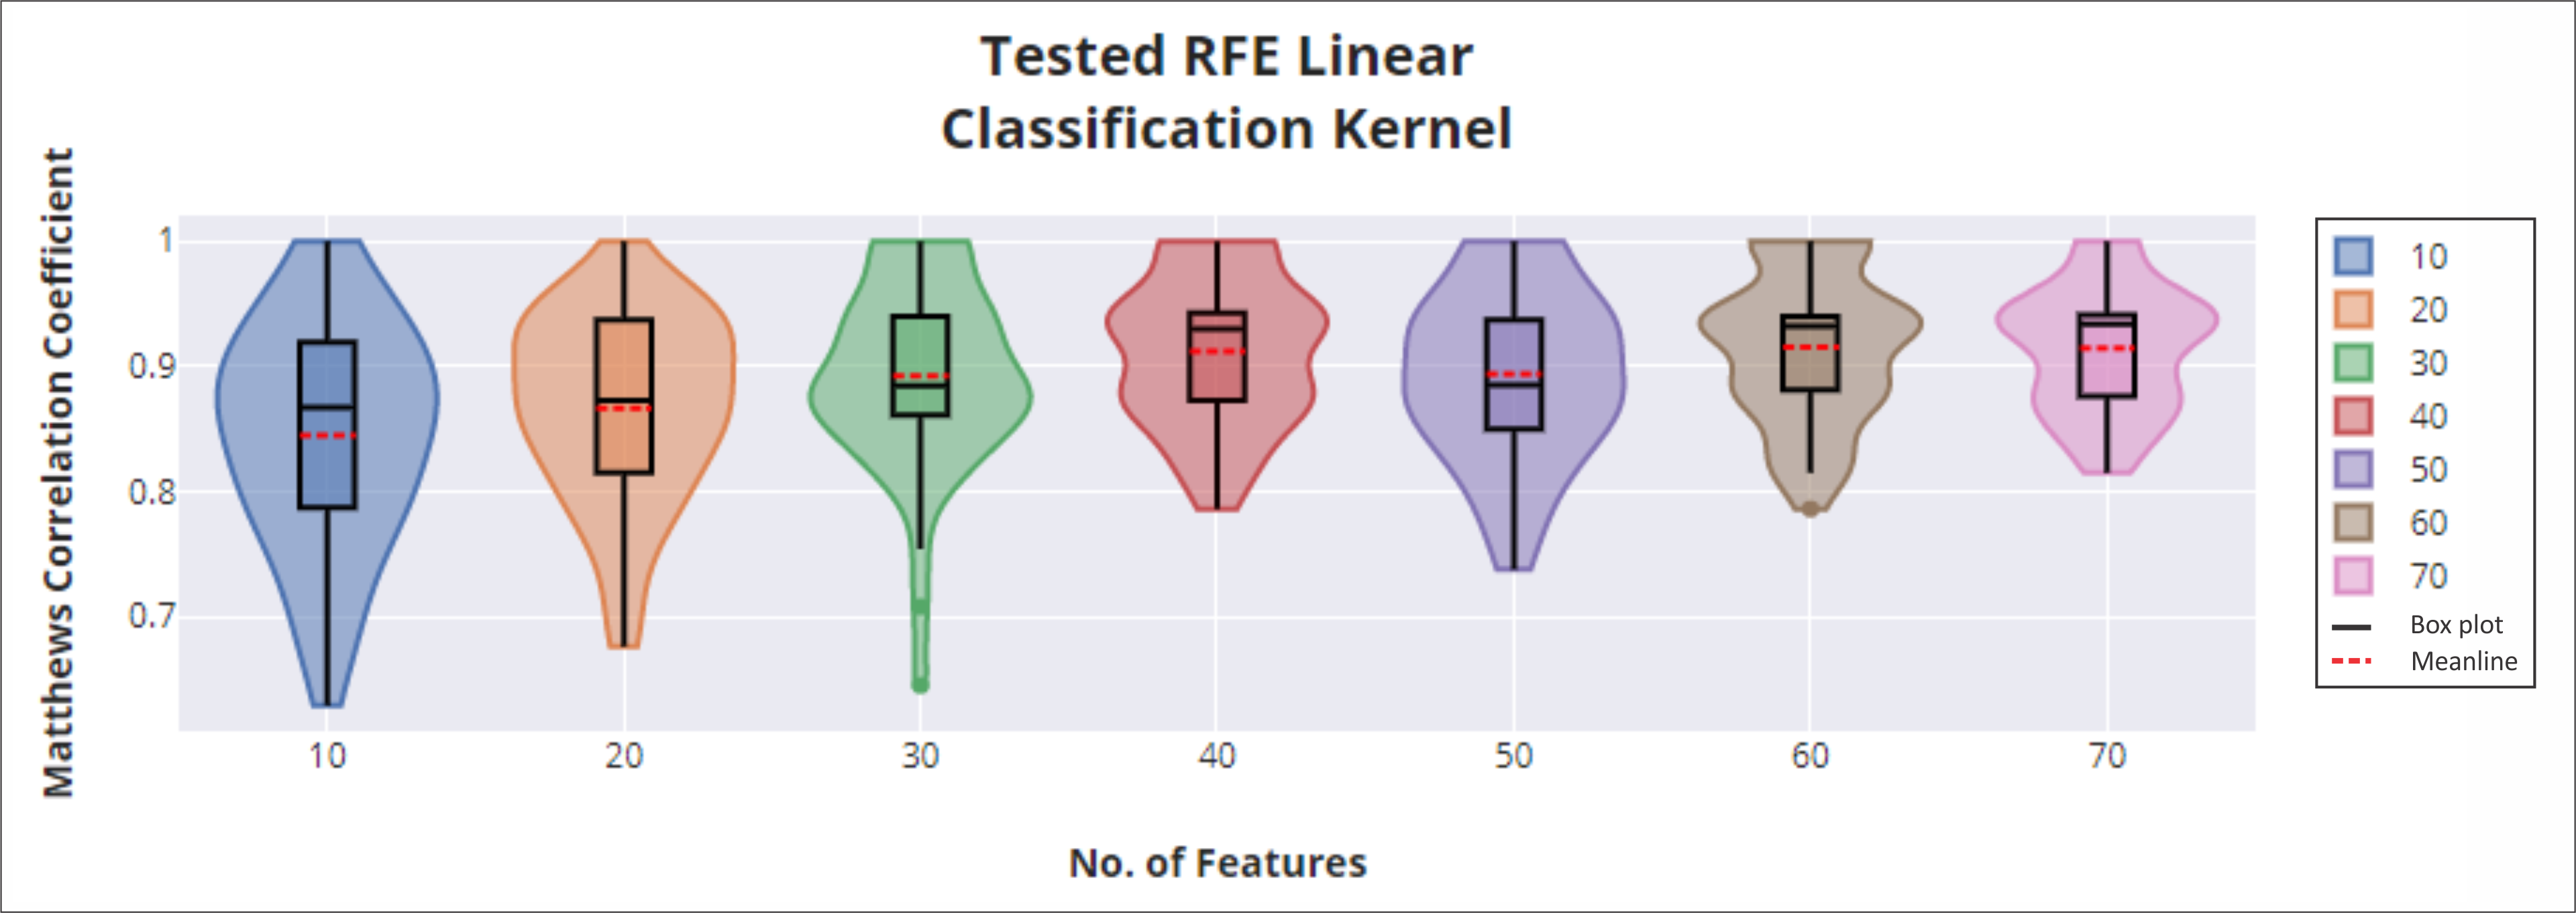
\includegraphics[width=500pt]{Tested_RFE_Linear_Classification_Kernel.PNG}
			\caption{Testing data: RFE linear classification kernel}
			\label{fig:Test_RFE_Linear}
		\end{center}
	\end{figure*}

		\begin{figure*}[h]
		\begin{center}
			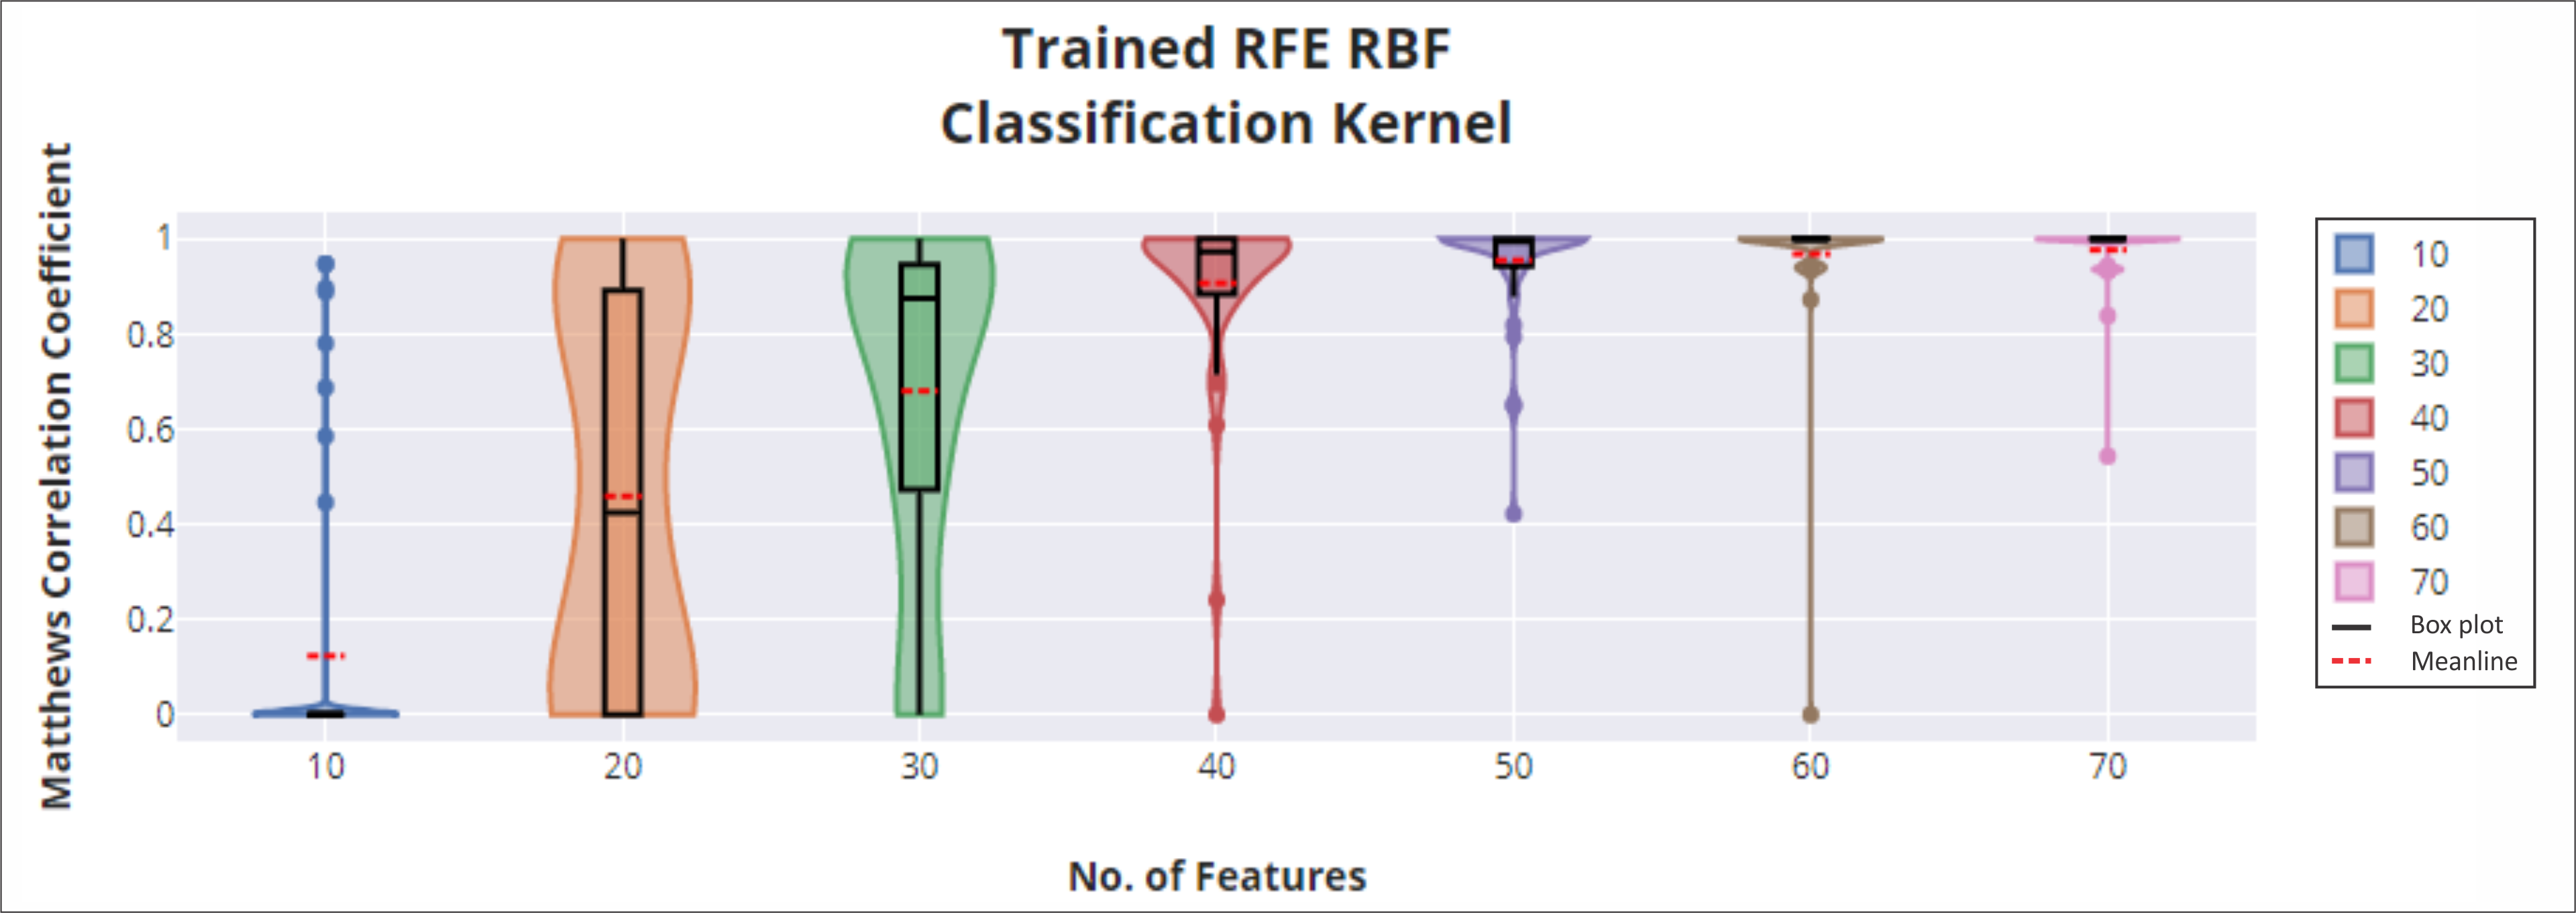
\includegraphics[width=500pt]{Trained_RFE_RBF_Classification_Kernel.PNG}
			\caption{Training data: RFE RBF classification kernel}
			\label{fig:Train_RFE_RBF}
		\end{center}
	\end{figure*}

		\begin{figure*}[h]
		\begin{center}
			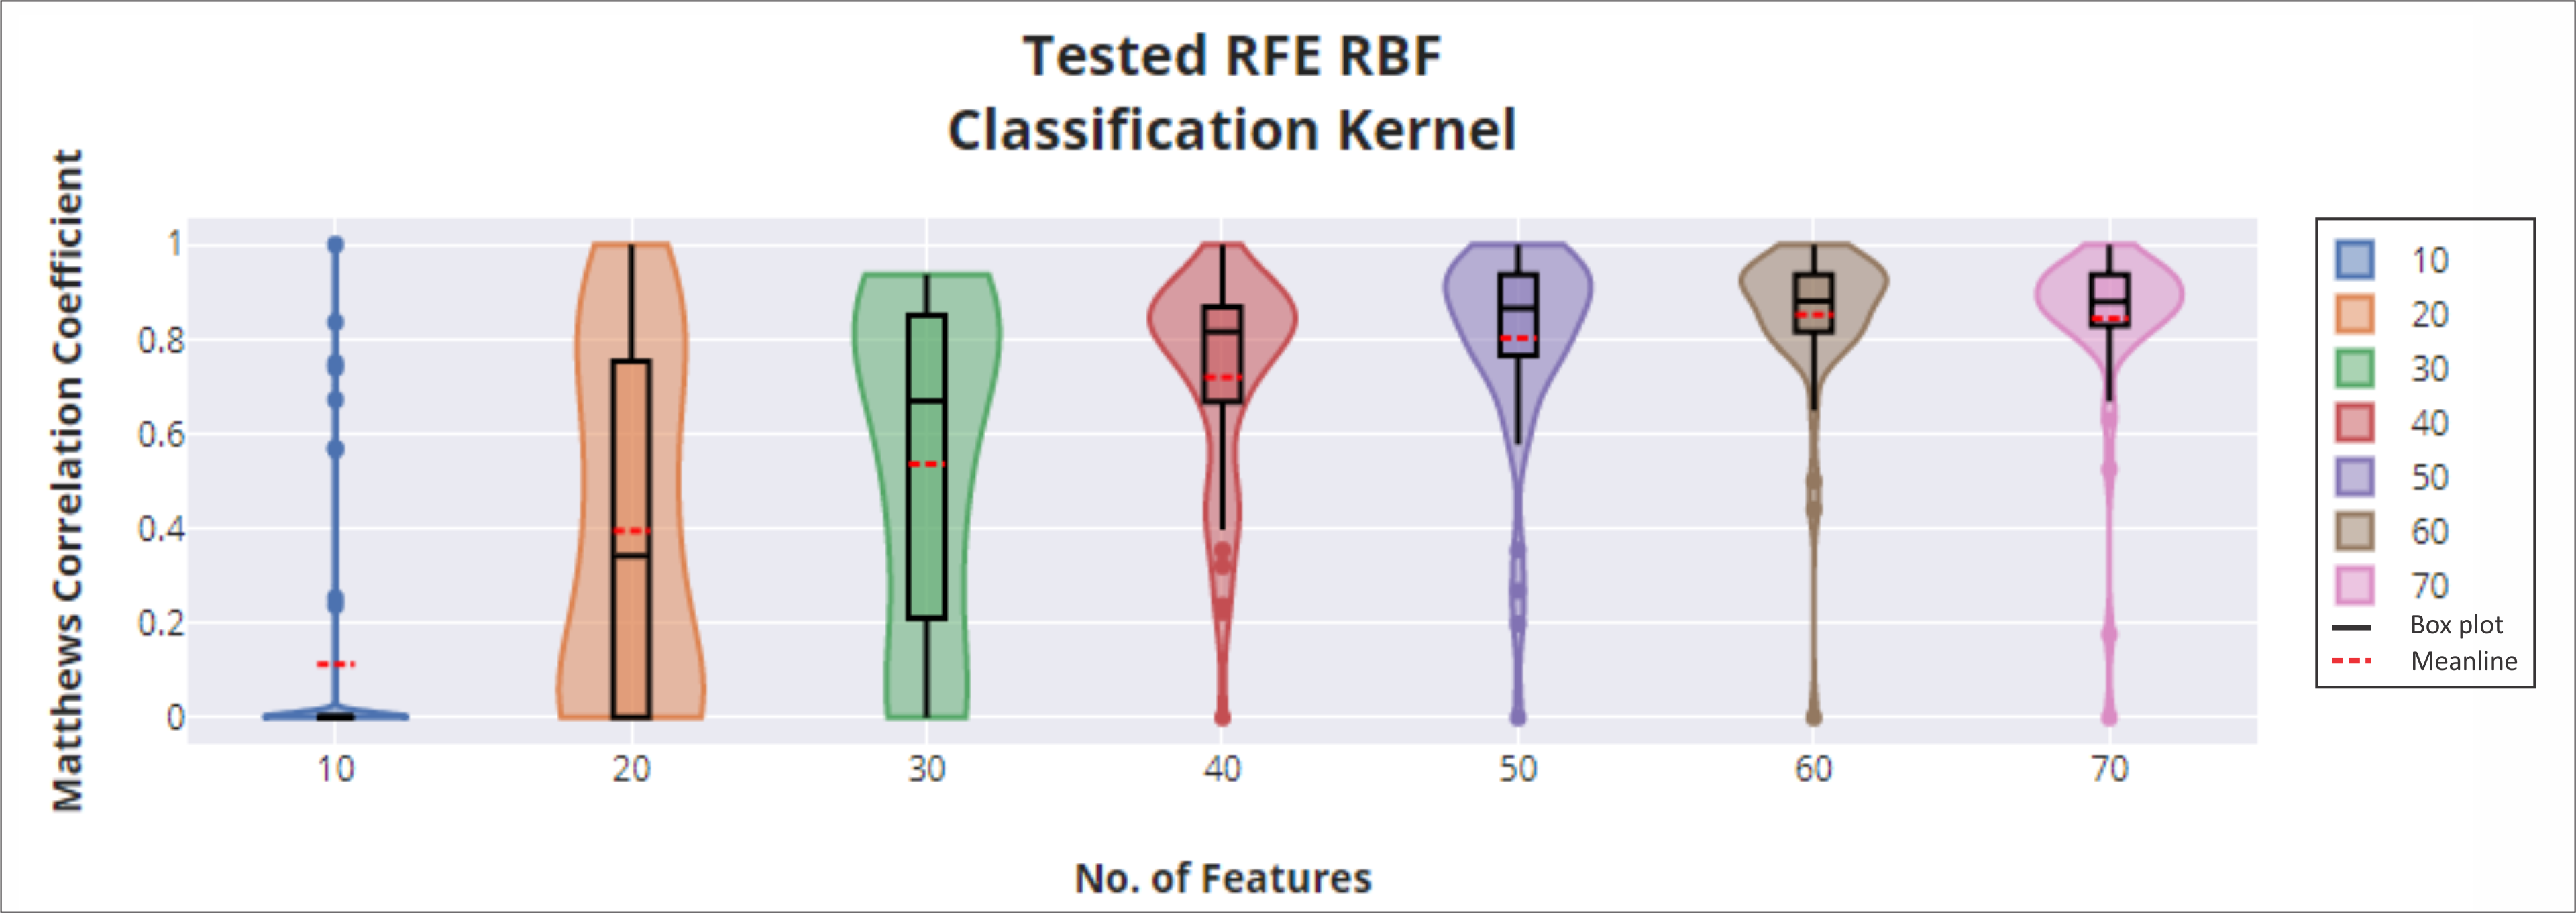
\includegraphics[width=500pt]{Tested_RFE_RBF_Classification_Kernel.PNG}
			\caption{Testing data: RFE RBF classification kernel}
			\label{fig:Test_RFE_RBF}
		\end{center}
	\end{figure*}

		\begin{figure*}[h]
		\begin{center}
			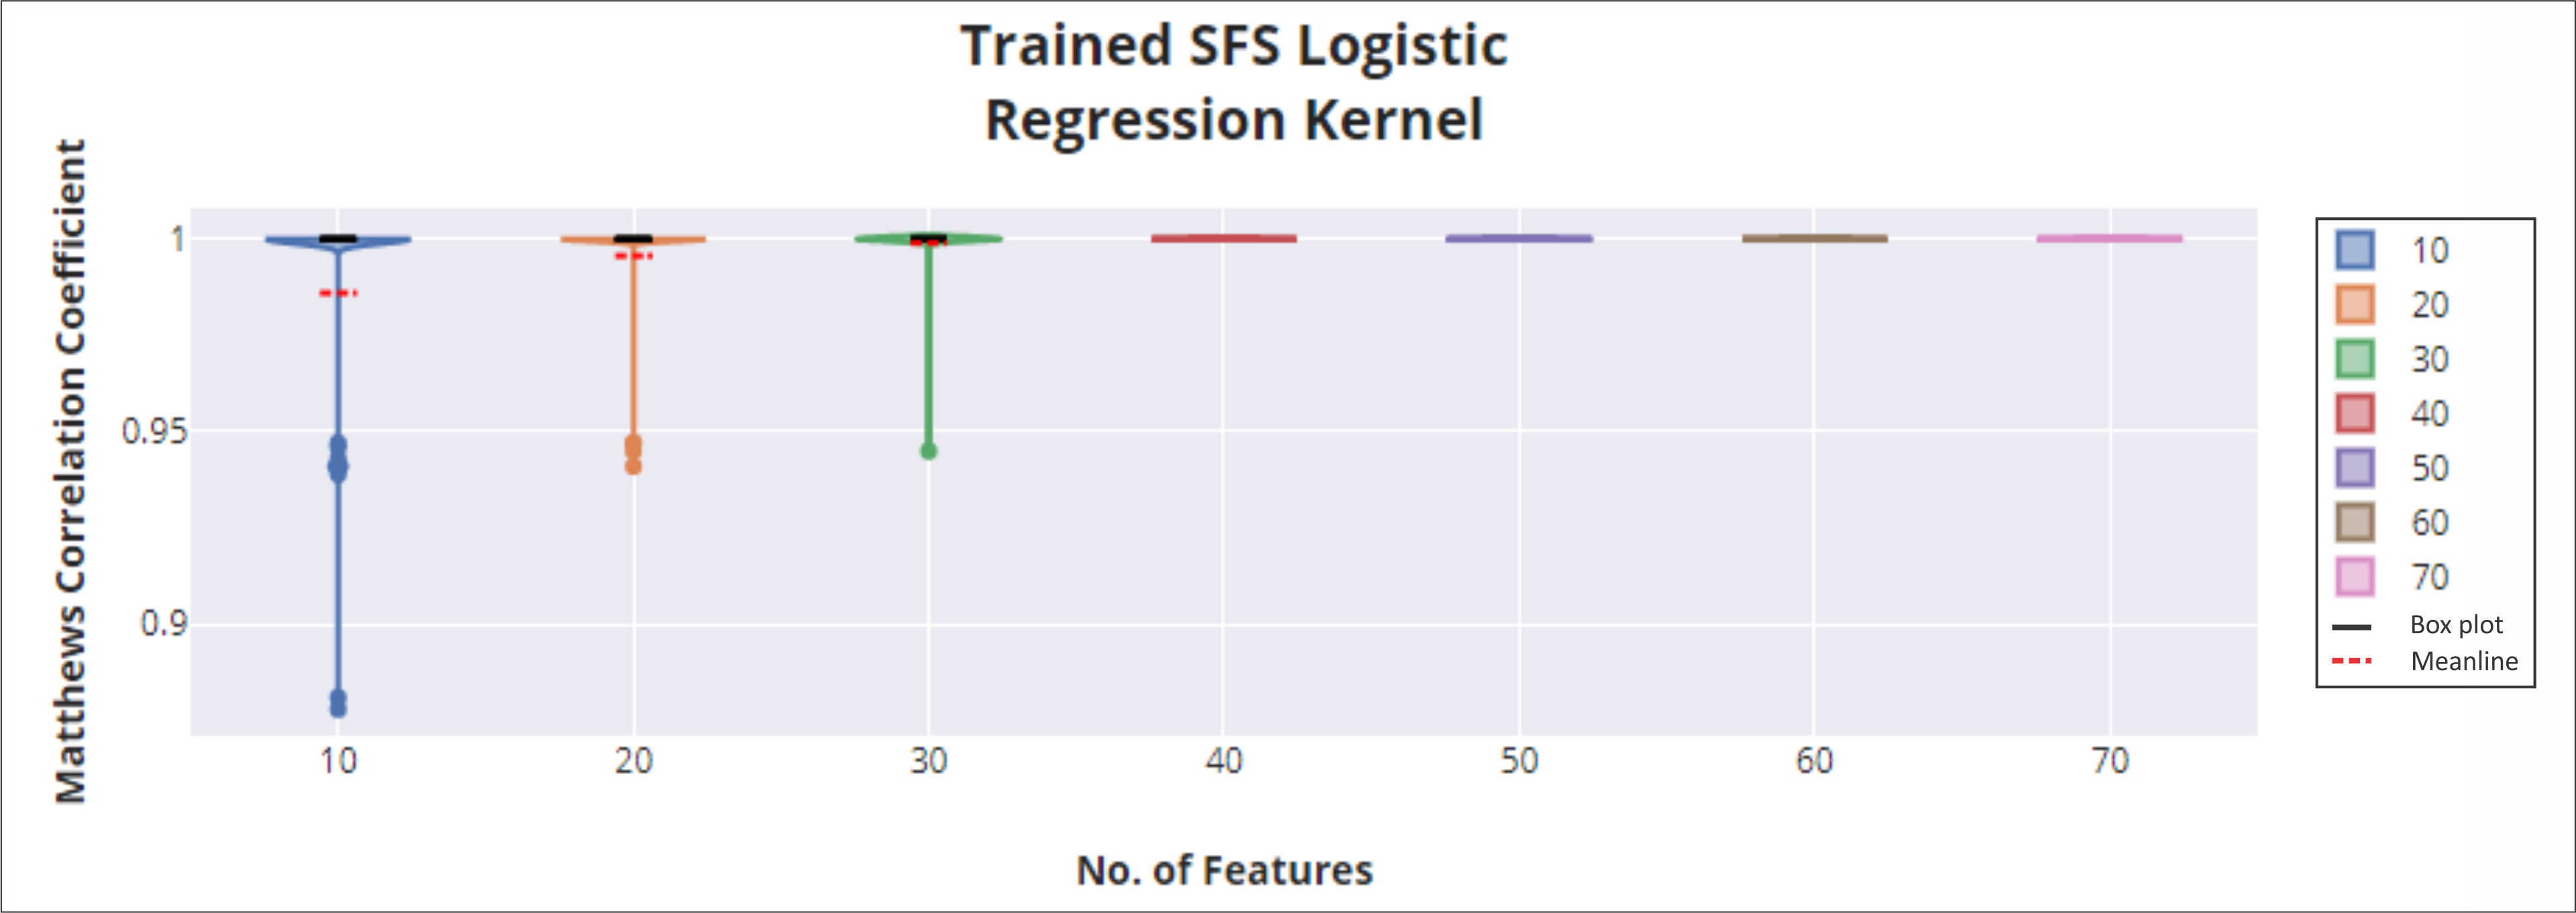
\includegraphics[width=500pt]{Trained_SFS_Logistic_Regression_Kernel.PNG}
			\caption{Training data: SFS Logistic Regression kernel}
			\label{fig:Train_SFS_Logistic}
		\end{center}
	\end{figure*}
	
		
		\begin{figure*}[h]
		\begin{center}
			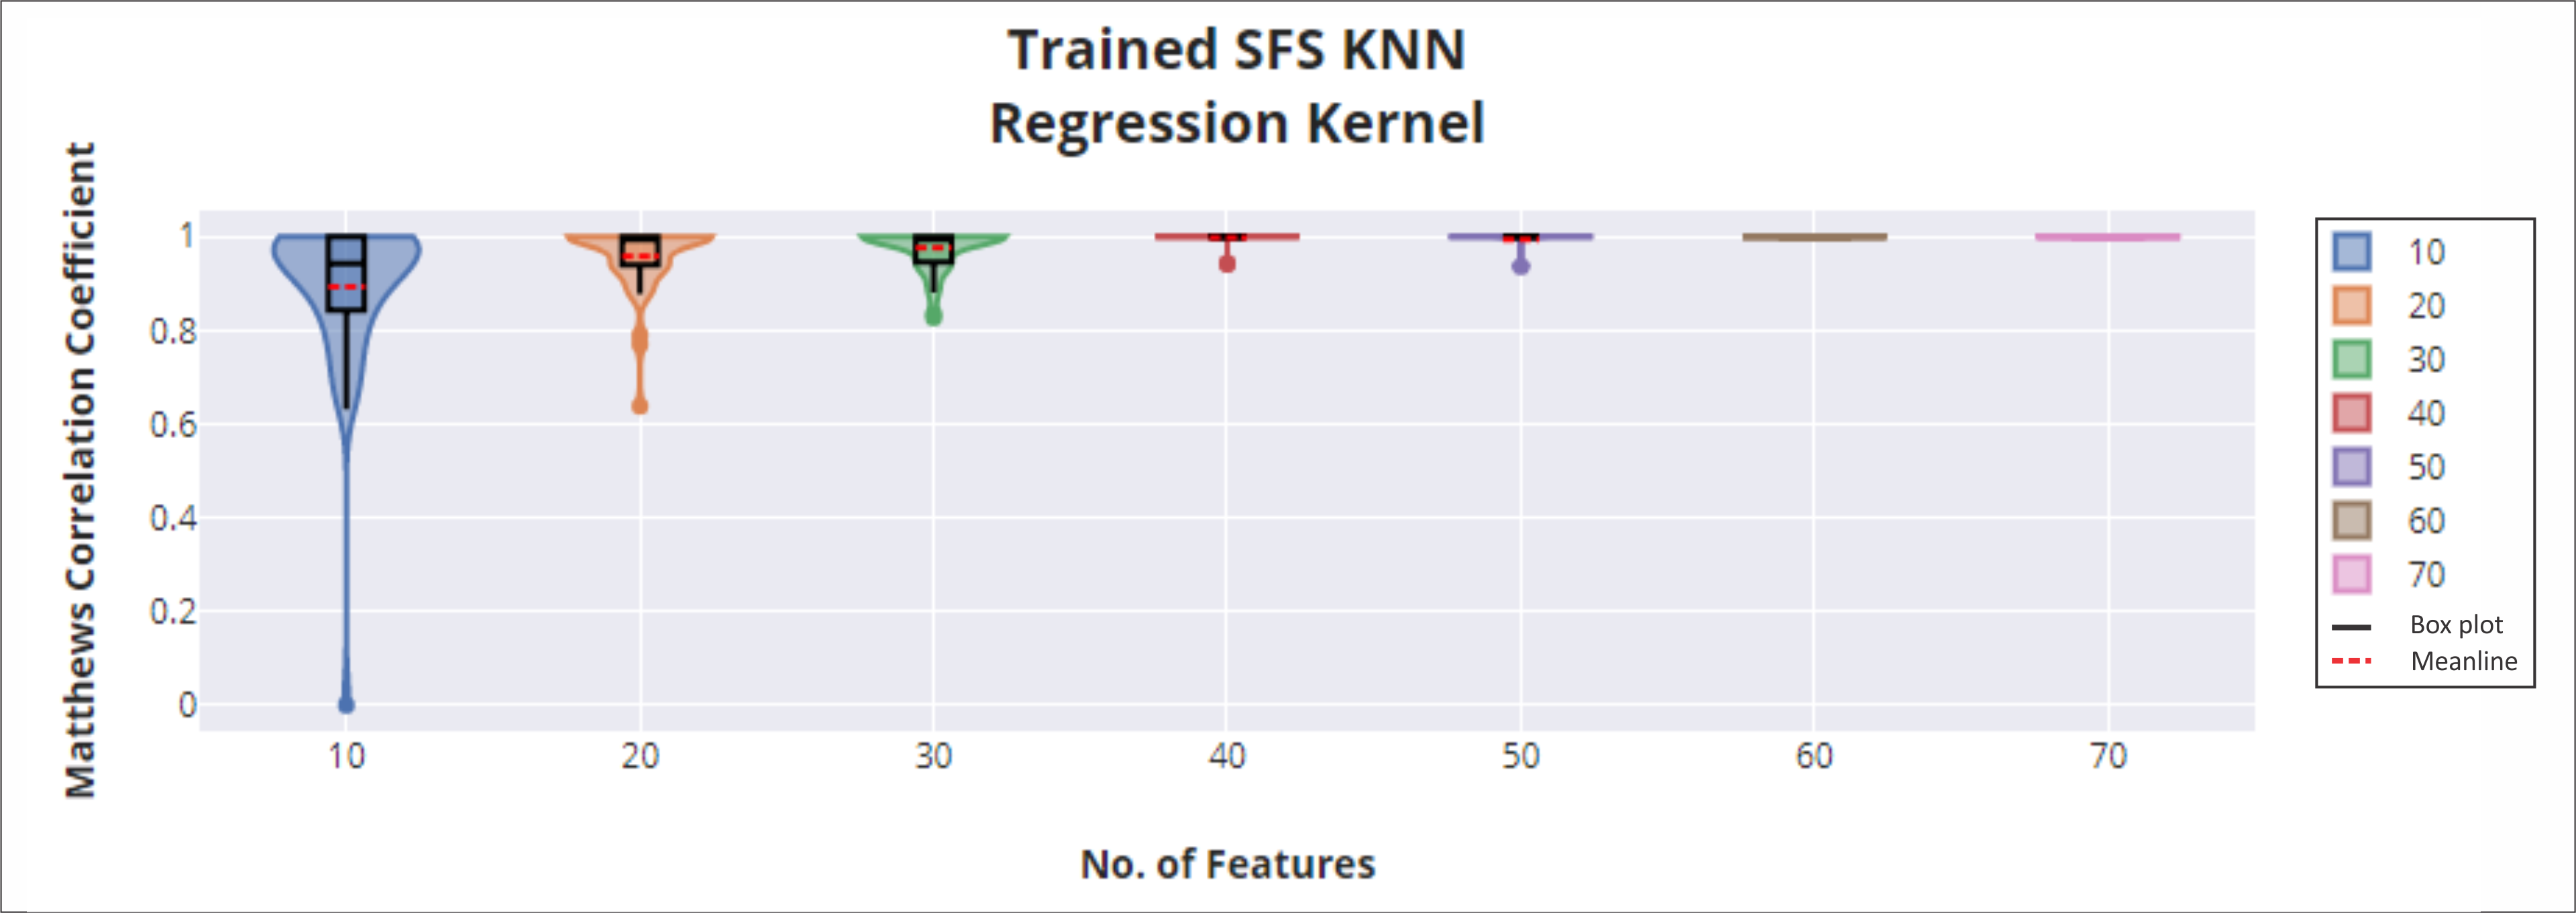
\includegraphics[width=500pt]{Trained_SFS_KNN_Regression_Kernel.PNG}
			\caption{Training data: SFS KNN Regression kernel}
			\label{fig:Train_SFS_KNN}
		\end{center}
	\end{figure*}
	
	
		\begin{figure*}[h]
		\begin{center}
			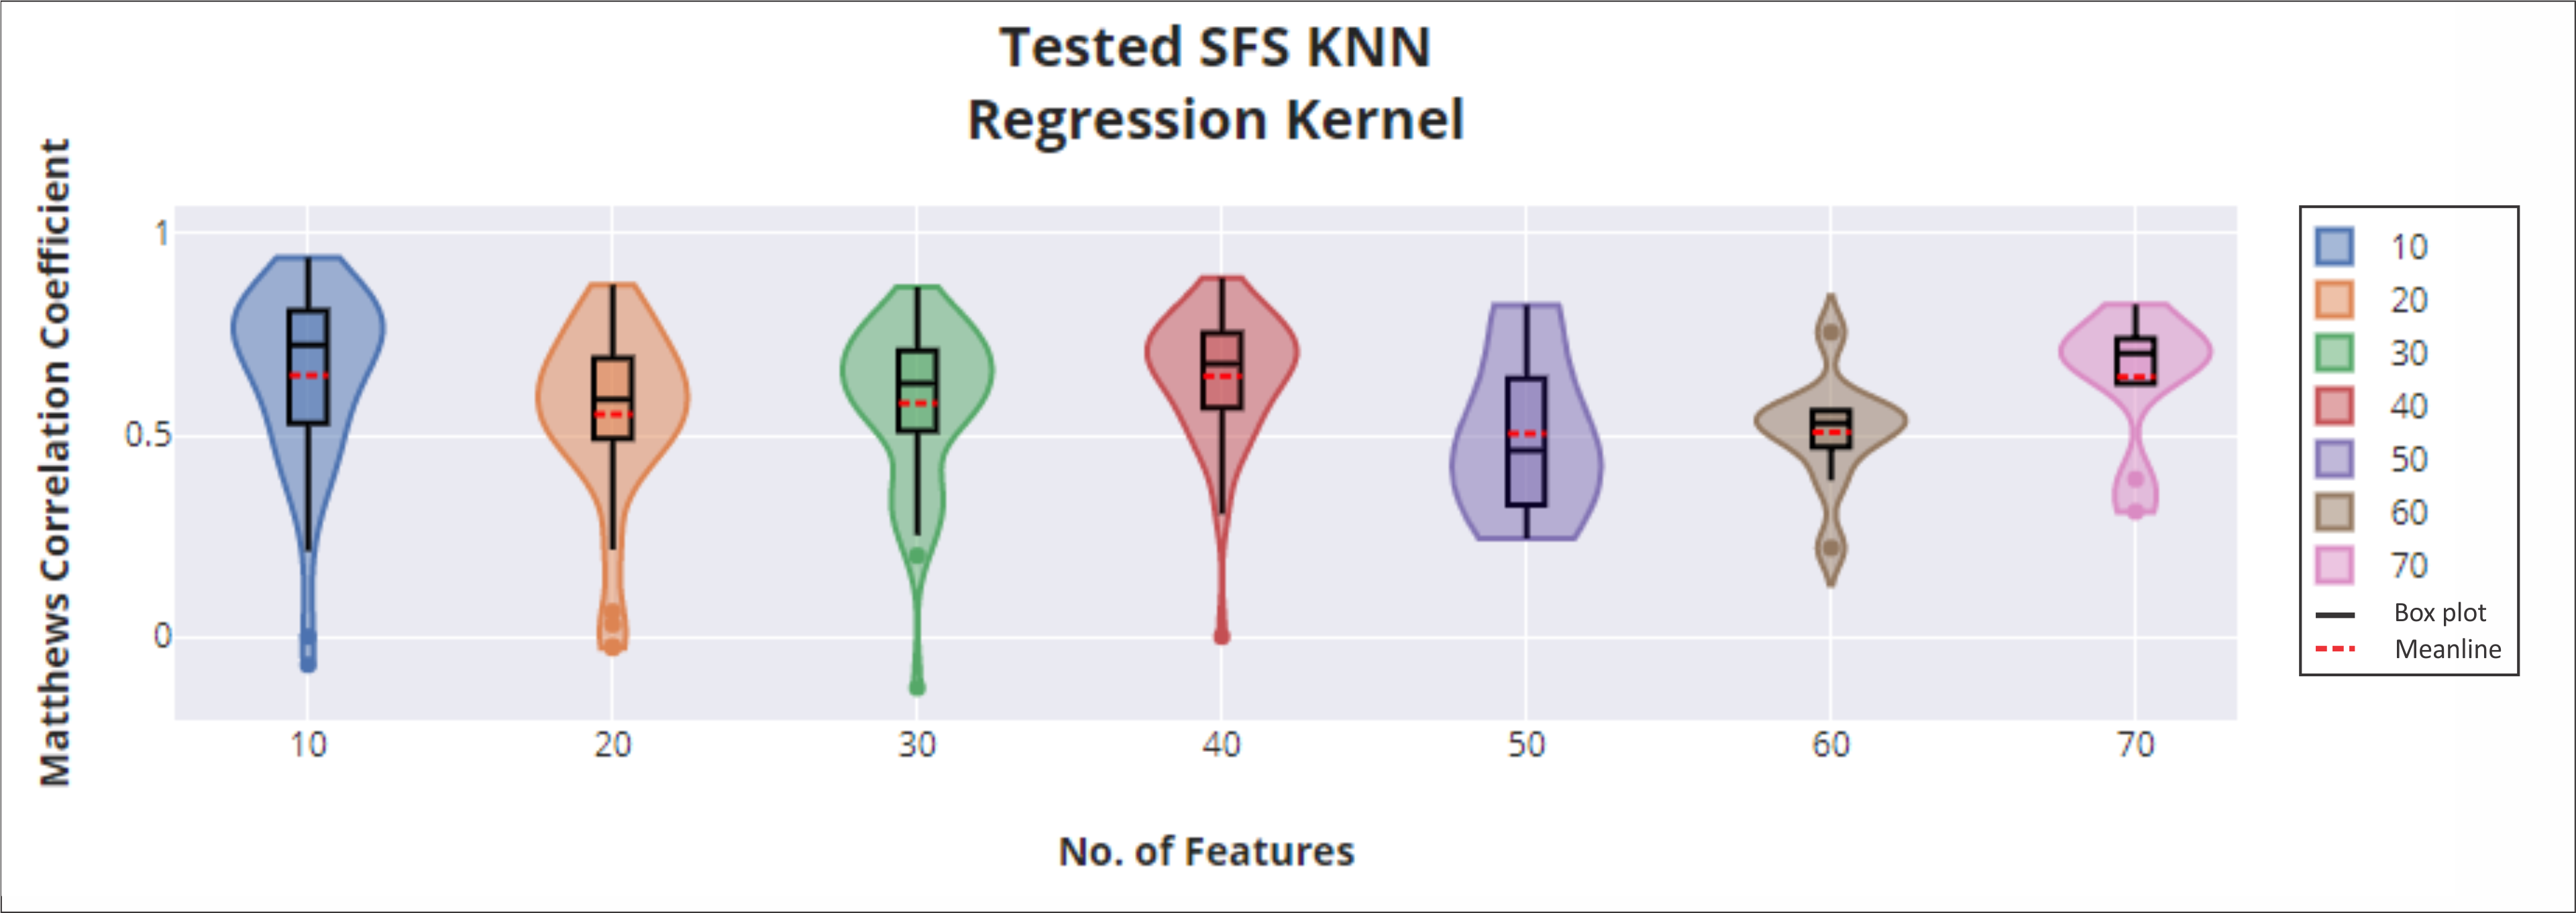
\includegraphics[width=500pt]{Tested_SFS_KNN_Regression_Kernel.PNG}
			\caption{Testing data: SFS KNN Regression kernel}
			\label{fig:Test_SFS_KNN}
		\end{center}
	\end{figure*}
	
		\begin{figure*}[h]
		\begin{center}
			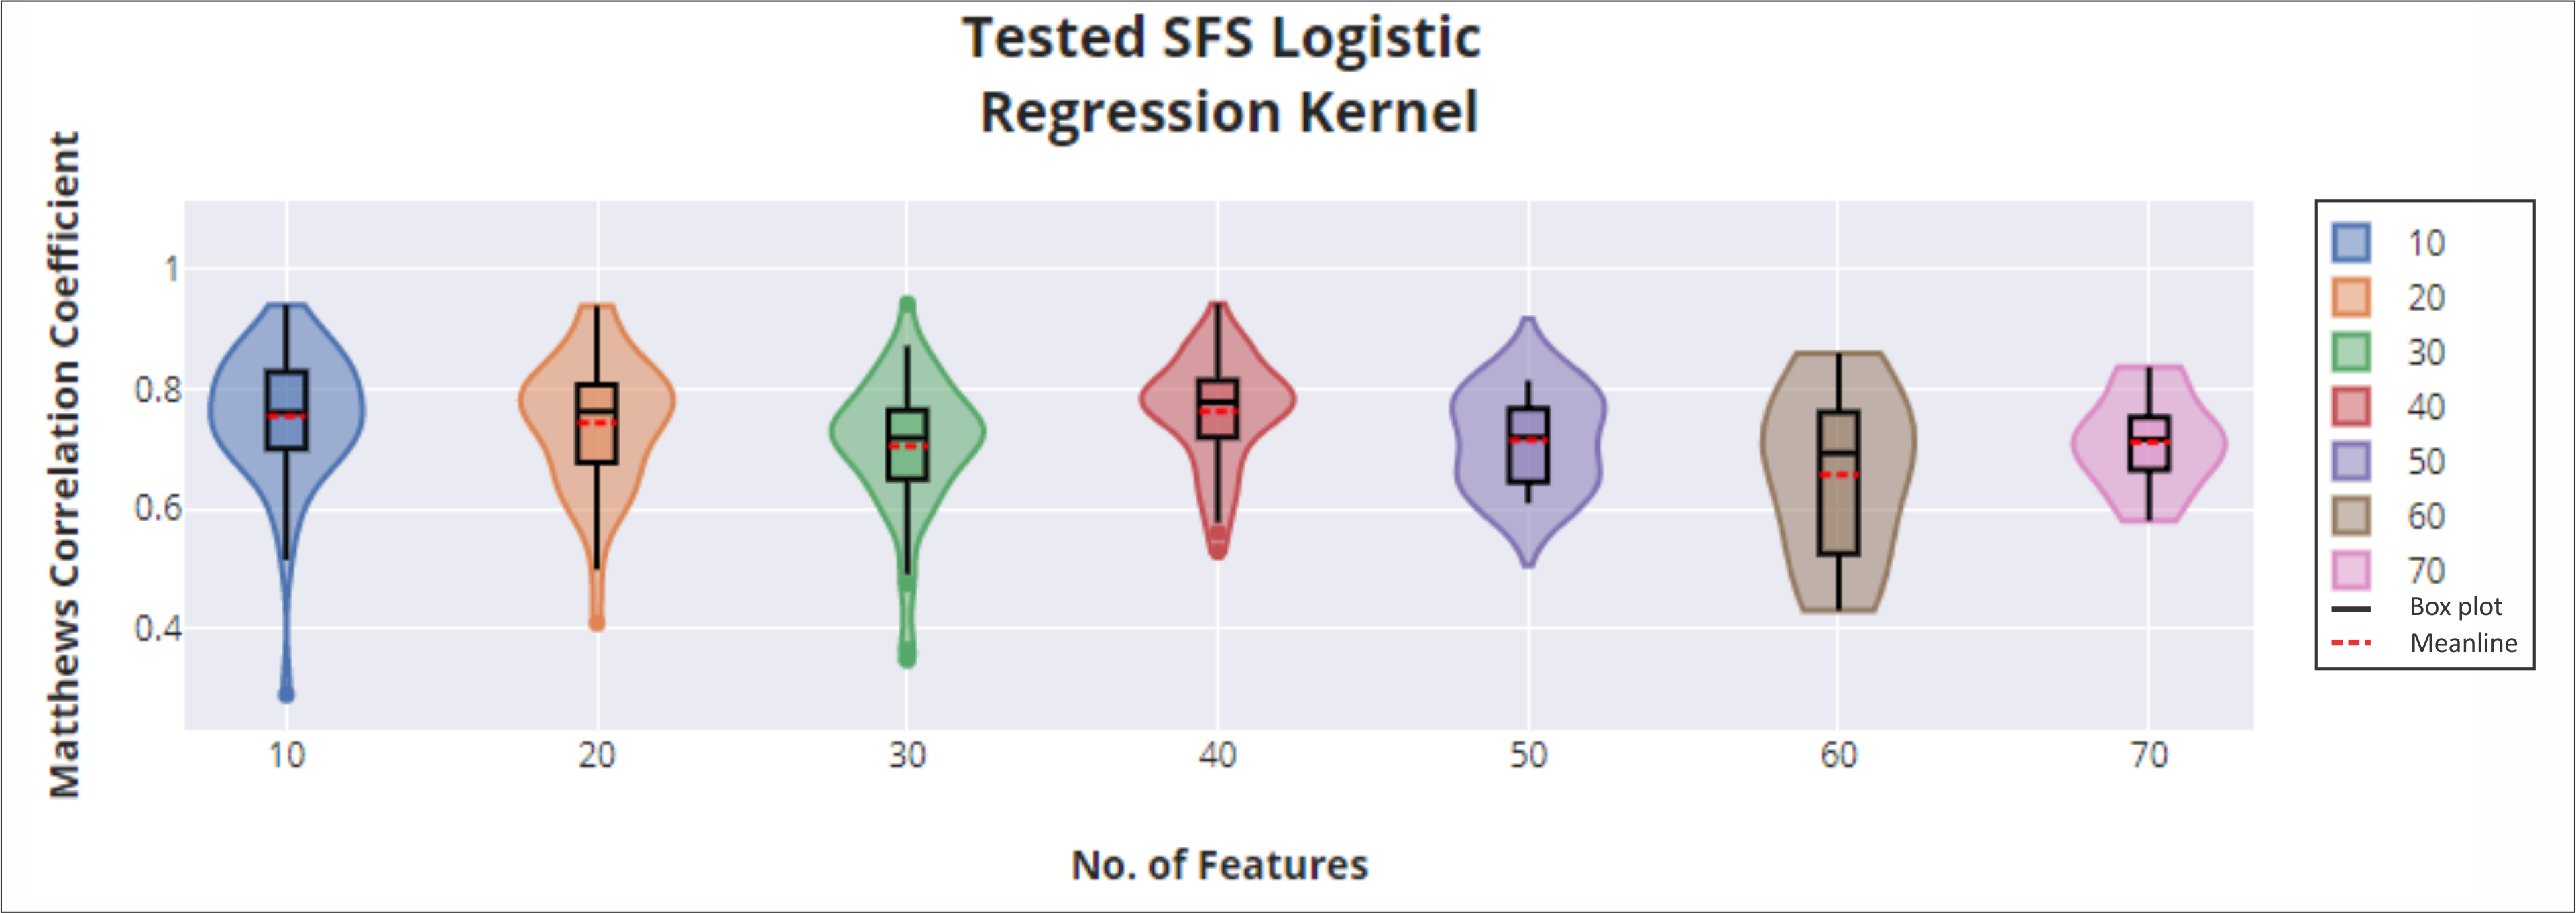
\includegraphics[width=500pt]{Tested_SFS_Logistic_Regression_Kernel.PNG}
			\caption{Testing data: SFS Logistic Regression kernel}
			\label{fig:Test_SFS_Logistic}
		\end{center}
	\end{figure*}
	
  %\begin{landscape}
	\begin{table*}[h]
	\caption{The average Matthew Correlation Coefficient (MCC) and average weighted accuracy of RFE and SFS with different kernel in different feature numbers}\label{tab:mcc_result}
\begin{tabular}{ccccccccc}

 \multicolumn{1}{c} { \multirow{3}{*}{Number of  features} } & \multicolumn{2}{c}{RFE Linear}                          & \multicolumn{2}{c}{RFE RBF}                             & \multicolumn{2}{c}{SFS KNN}                             & \multicolumn{2}{c}{SFS Logistic}                        \\
       \multicolumn{1}{c}{}         & \multicolumn{2}{c}{Classification Kernel}               & \multicolumn{2}{c}{Classification Kernel}               & \multicolumn{2}{c}{Regression Kernel}                   & \multicolumn{2}{c}{Regression Kernel}                   \\ \cline{2-9} 
           \multicolumn{1}{c}{}             & \multicolumn{1}{c}{MCC} & \multicolumn{1}{c}{Accuracy} & \multicolumn{1}{c}{MCC} & \multicolumn{1}{c}{Accuracy} & \multicolumn{1}{c}{MCC} & \multicolumn{1}{c}{Accuracy} & \multicolumn{1}{c}{MCC} & \multicolumn{1}{c}{Accuracy} \\ \cline{2-9} 
10  & 0.84   & 92.80\%  & 0.11  & 44.18\%  & 0.64 & 84.46\% & 0.75 & 89.52\%  \\
20  & 0.86   & 94.02\%  & 0.39  & 68.78\%  & 0.55 & 79.51\% & 0.74 & 89.16\% \\
30  & 0.89   & 95.42\%  & 0.53  & 78.26\%  & 0.57 & 81.74\% & 0.70 & 86.36\% \\
40  & 0.91   & 95.57\%  & 0.71  & 89.85\%  & 0.64 & 84.06\% & 0.76 & 89.94\% \\
50  & 0.89   & 95.55\%  & 0.80  & 92.38\%  & 0.50 & 76.93\% & 0.71 & 86.39\% \\
60  & 0.91   & 96.24\%  & 0.85  & 93.41\%  & 0.50 & 77.50\% & 0.65 & 84.57\% \\
70  & 0.91   & 96.16\%  & 0.84  & 92.86\%  & 0.64 & 83.96\% & 0.71 & 86.35\% \\
80  & 0.91   & 96.24\%  & 0.87  & 94.81\%  & 0.62 & 83.36\% & 0.64 & 83.93\% \\
90  & 0.92   & 96.61\%  & 0.89  & 95.76\%  & 0.67 & 84.82\% & 0.71 & 87.07\% \\
100 & 0.91   & 95.78\%  & 0.91  & 95.98\%  & 0.58 & 81.43\% & 0.73 & 88.79\% \\
110 & 0.92   & 96.46\%  & 0.88  & 95.28\%  & 0.72 & 87.00\% & 0.73 & 88.04\% \\
120 & 0.91   & 96.01\&  & 0.90  & 95.74\%  & 0.68 & 86.07\% & 0.72 & 87.75\% \\
130 & 0.92   & 96.28\%  & 0.91  & 96.18\%  & 0.71 & 87.86\% & 0.73 & 88.75\% \\
140 & 0.91   & 96.18\%  & 0.92  & 96.26\%  & 0.66 & 83.50\% & 0.80 & 91.82\% \\
\end{tabular}
\end{table*}
%\end{landscape}

	\begin{figure*}[hb]
		\begin{center}
			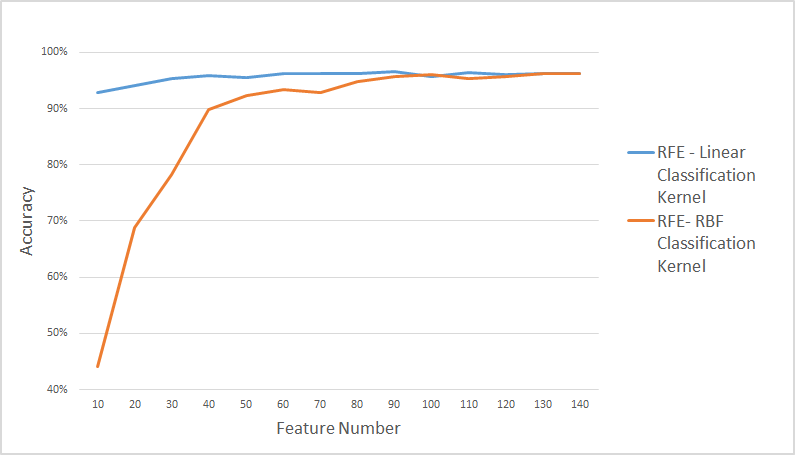
\includegraphics[width=230pt]{RFE_accuracy.png}
			\caption{RFE prediction accuracy in different feature number}
			\label{fig:RFE_accuracy}
		\end{center}
	\end{figure*}
	
		\begin{figure*}[hb]
		\begin{center}
			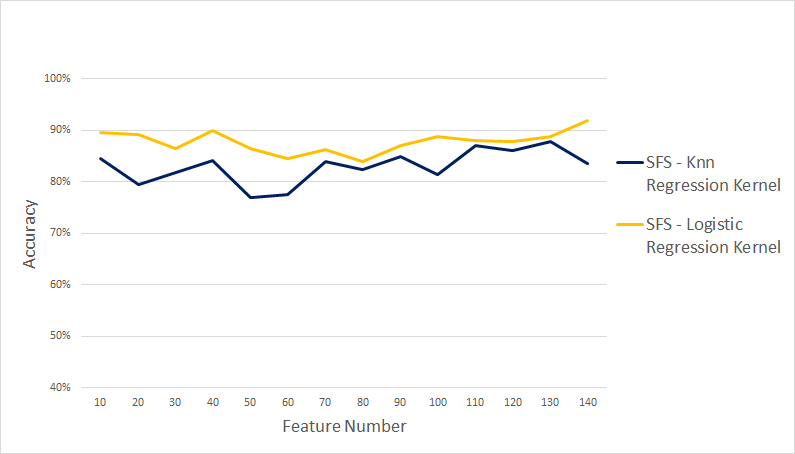
\includegraphics[width=230pt]{SFS_accuracy.png}
			\caption{SFS prediction accuracy in different feature number}
			\label{fig:SFS_accuracy}
		\end{center}
	\end{figure*}


\end{document}